% This file is used as input to the main file.

\bisection{Feria Sexta}{Friday}\label{Friday}

\bisubsectionnoline{Psalmus 87 \textemdash{} Hominis graviter ægrotantis oratio}{Psalm 87 \textemdash{} The prayer of one gravely ill}

\bisentence{“Hæc est hora vestra et potestas tenebrarum” \textup{(Lc 22, 53).}}{“This is your hour; this is the reign of darkness” \textup{(Lk 22:53).}}

\bimusic{\gregorioscore{../AntiphonsAndPsalmsAndReadings/6Friday/11239-an--domine_deus_salutis_(mode_3b)--verona,H6C1.gabc}}{\GreColored{Ant.} Lord God of my salvation, I call for help by day, I cry at night before you.}

\verticalspacer

\biinstruction{Vel, ad libitum antiphona \textcolor{black}{Domine, Deus salutis} in alio tono dici potest, quæ cum \textcolor{black}{Psalmo 87} secundum antiphonam invenitur post lectionem brevem.}{Or, when desired, \textcolor{black}{Domine, Deus salutis} can be sung with a different tone, which is found after the reading with \textcolor{black}{Psalm 87} conforming to the antiphon.}

\bimusic[Vel, in tempore paschali:][Or, in Easter time:]{\gregorioscore{../AntiphonsAndPsalmsAndReadings/6Friday/3000-an--alleluia._(sund._p._t._at_prime)--solesmes_1961-no-signs.gabc}}{\GreColored{Ant.} Alleluia, alleluia, alleluia.}

\bireading{\gregorioscore{../AntiphonsAndPsalmsAndReadings/6Friday/88-3b.gabc}}{\gregorioscore{../AntiphonsAndPsalmsAndReadings/6Friday/88-3b-en.gabc}}

\verticalspacerpsalm

\bihangingpsalm{
Intret in conspéctu tuo o\textbf{rá}tio \textbf{me}a;\redstar\\
inclína aurem tuam ad \textbf{pre}cem \textbf{me}am.

Quia repléta est malis \textbf{á}nima \textbf{me}a,\redstar\\
et vita mea inférno ap\textbf{pro}pin\textbf{quá}vit.

Æstimátus sum cum descendénti\textbf{bus} in \textbf{la}cum,\redstar\\
factus sum sicut homo sine \textbf{ad}iu\textbf{tó}rio.

Inter \textbf{mór}tuos \textbf{li}ber,\redstar\\
sicut vulneráti dormiéntes \textbf{in} se\textbf{púl}cris;

quorum non es \textbf{me}mor \textbf{ámpli}us,\redstar\\
et ipsi de manu \textbf{tu}a ab\textbf{scís}si sunt.

Posuísti me in lacu in\textbf{fe}ri\textbf{ó}ri,\redstar\\
in tenebrósis et in \textbf{um}bra \textbf{mor}tis.

Super me gravátus est \textbf{fu}ror \textbf{tu}us,\redstar\\
et omnes fluctus tuos indu\textbf{xís}ti \textbf{su}per me.

Longe fecísti notos \textbf{me}os \textbf{a} me,\redstar\\
posuísti me abominati\textbf{ó}nem \textbf{e}is;

conclúsus sum et \textbf{non} e\textbf{grédi}ar.\redstar\\
Oculi mei languérunt præ af\textbf{flic}ti\textbf{ó}ne.

Clamávi ad te, Dómine, \textbf{to}ta \textbf{di}e,\redstar\\
expándi ad te \textbf{ma}nus \textbf{me}as.

Numquid mórtuis fácies \textbf{mi}ra\textbf{bíli}a,\redstar\\
aut surgent umbræ et confite\textbf{bún}tur \textbf{ti}bi?

Numquid narrábit áliquis in sepúlcro miseri\mbox{\textbf{cór}diam \textbf{tu}am\redstar}\\
et veritátem tuam in loco per\textbf{di}ti\textbf{ó}nis?

Numquid cognoscéntur in ténebris mira\textbf{bí}lia \textbf{tu}a,\redstar\\
et iustítia tua in terra ob\textbf{li}vi\textbf{ó}nis?

Et ego ad te, Dómi\textbf{ne}, cla\textbf{má}vi,\redstar\\
et mane orátio mea præ\textbf{vé}ni\textbf{et} te.

Ut quid, Dómine, repéllis \textbf{á}nimam \textbf{me}am,\redstar\\
abscóndis fáciem \textbf{tu}am \textbf{a} me?

Pauper sum ego et móriens a iuven\textbf{tú}te \textbf{me}a;\redstar\\
portávi pavóres tuos et \textbf{con}tur\textbf{bá}tus sum.

Super me transiérunt \textbf{i}ræ \textbf{tu}æ,\redstar\\
et terróres tui \textbf{ex}ci\textbf{dé}runt me.

Circuiérunt me sicut aqua \textbf{to}ta \textbf{di}e,\redstar\\
circumde\textbf{dé}runt me \textbf{si}mul.

Elongásti a me a\textbf{mí}cum et \textbf{próxi}mum,\redstar\\
et noti \textbf{me}i sunt \textbf{té}nebræ.

Glória \textbf{Pa}tri, et \textbf{Fíli}o,\redstar\\
et Spi\textbf{rí}tui \textbf{Sanc}to.

Sicut erat in princípio, et \textbf{nunc}, et \textbf{sem}per,\redstar\\
et in sǽcula sæcu\textbf{ló}rum. \textbf{A}men.
}
{
Let my prayer come \textbf{in}to your \textbf{pre}sence.\redstar\\
O turn your \textbf{ear} to \textbf{my} cry.

For my soul is \textbf{filled} with \textbf{e}vils;\redstar\\
my life is on the \textbf{brink} of \textbf{the} grave.

I am reckoned as \textbf{one} in \textbf{the} tomb:\redstar\\
I have reached the \textbf{end} of \textbf{my} strength,

like one a\textbf{lone} a\textbf{mong the} dead;\redstar\\
like the slain \textbf{ly}ing \textbf{in} their graves;

like those you re\textbf{mem}ber \textbf{no} more,\redstar\\
cut off, as they \textbf{are}, from \textbf{your} hand.

You have laid me in the \textbf{depths} of \textbf{the} tomb,\redstar\\
in places that are \textbf{dark}, in \textbf{the} depths.

Your anger \textbf{weighs} down u\textbf{pon} me:\redstar\\
I am \textbf{drowned} be\textbf{neath} your waves.

You have \textbf{tak}en a\textbf{way my} friends\redstar\\
and made me \textbf{hate}ful \textbf{in} their sight.

Imprisoned, I \textbf{can}not \textbf{es}cape;\redstar\\
my eyes are \textbf{sun}ken \textbf{with} grief.

I call to you, Lord, \textbf{all} the \textbf{day} long;\redstar\\
to you I \textbf{stretch} out \textbf{my} hands.

Will you work your \textbf{won}ders \textbf{for the} dead?\redstar\\
Will the shades \textbf{stand} and \textbf{praise} you?

Will your \textbf{love} be told \textbf{in the} grave\redstar\\
or your faithful\textbf{ness} a\textbf{mong} the dead?

Will your wonders be \textbf{known} in \textbf{the} dark\redstar\\
or your justice in the \textbf{land} of ob\textbf{li}vion?

As for me, Lord, I \textbf{call} to you \textbf{for} help:\redstar\\
in the morning my \textbf{prayer} comes be\textbf{fore} you.

Lord, why \textbf{do} you re\textbf{ject} me?\redstar\\
Why \textbf{do} you \textbf{hide} your face?

Wretched, close to \textbf{death} from \textbf{my} youth,\redstar\\
I have \textbf{borne} your trials; \textbf{I} am numb.

Your fury has swept \textbf{down} u\textbf{pon} me;\redstar\\
your terrors have utter\textbf{ly} de\textbf{stroyed} me.

They surround me all the \textbf{day} like \textbf{a} flood,\redstar\\
they assail me \textbf{all} to\textbf{ge}ther.

Friend and neighbour you have \textbf{ta}ken \textbf{a}way:\redstar\\
my one com\textbf{pan}ion is \textbf{dark}ness.

Glory be to the \textbf{Fa}ther and \textbf{to the} Son\redstar\\
and to the \textbf{Ho}ly \textbf{Spi}rit,

as it was in the beginning, is now, and \textbf{e}ver \textbf{shall} be,\redstar\\
world with\textbf{out} end. \textbf{A}men.
}

\bimusic{\gregorioscore{../AntiphonsAndPsalmsAndReadings/6Friday/11239-an--domine_deus_salutis_(mode_3b)--verona,H6C1.gabc}}{\GreColored{Ant.} Lord God of my salvation, I call for help by day, I cry at night before you.}

\bimusic[Vel, in tempore paschali:][Or, in Easter time:]{\gregorioscore{../AntiphonsAndPsalmsAndReadings/6Friday/3000-an--alleluia._(sund._p._t._at_prime)--solesmes_1961-no-signs.gabc}}{\GreColored{Ant.} Alleluia, alleluia, alleluia.}

\vspace{-0.2cm}
\bisubsection{Lectio brevis \textemdash{} cf. Ier 14}{Short reading \textemdash{} cf. Jer 14}
\vspace{-0.2cm}

\bireading{\gregorioscore{../AntiphonsAndPsalmsAndReadings/6Friday/FridayLectioBrevis.gabc}}{\gregorioscore{../AntiphonsAndPsalmsAndReadings/6Friday/FridayLectioBrevis-en.gabc}}

\vspace{-0.2cm}
\verticalspacer

\biinstruction{Responsorium breve subsequitur, p. \textcolor{black}{\pageref{ResponsoriumBreve}.}}{The short response follows, p. \textcolor{black}{\pageref{ResponsoriumBreve}.}}

\redlineseparator

% \newpage

\bisubsection{Psalmus 87 \textemdash{} Hominis graviter ægrotantis oratio (in alio tono)}{Psalm 87 \textemdash{} The prayer of one gravely ill (in a different tone)}

\bisentence{“Hæc est hora vestra et potestas tenebrarum” \textup{(Lc 22, 53).}}{“This is your hour; this is the reign of darkness” \textup{(Lk 22:53).}}

\bimusic{\gregorioscore{../AntiphonsAndPsalmsAndReadings/6Friday/11240-an--domine_deus_salutis_(mode_4*e)--verona,H6C1.gabc}}{\GreColored{Ant.} Lord God of my salvation, I call for help by day, I cry at night before you.}

\bireading{\gregorioscore{../AntiphonsAndPsalmsAndReadings/6Friday/88-4.gabc}}{\gregorioscore{../AntiphonsAndPsalmsAndReadings/6Friday/88-4-en.gabc}}

\verticalspacerpsalm

\bihangingpsalm{
Intret in conspéctu tuo orá\textit{tio} \textbf{me}a;\redstar\\
inclína aurem tuam ad \textbf{pre}cem \textbf{me}am.

Quia repléta est malis á\textit{nima} \textbf{me}a,\redstar\\
et vita mea inférno ap\textbf{pro}pin\textbf{quá}vit.

Æstimátus sum cum descendénti\textit{bus} \textit{in} \textbf{la}cum,\redstar\\
factus sum sicut homo sine \textbf{ad}iu\textbf{tó}rio.

Inter mór\textit{tuos} \textbf{li}ber,\redstar\\
sicut vulneráti dormiéntes \textbf{in} se\textbf{púl}cris;

quorum non es \textit{memor} \textbf{ám}plius,\redstar\\
et ipsi de manu \textbf{tu}a ab\textbf{scís}si sunt.

Posuísti me in lacu in\textit{feri}\textbf{ó}ri,\redstar\\
in tenebrósis et in \textbf{um}bra \textbf{mor}tis.

\newpage

Super me gravátus est \textit{furor} \textbf{tu}us,\redstar\\
et omnes fluctus tuos indu\textbf{xís}ti \textbf{su}per me.

Longe fecísti notos \textit{meos} \textbf{a} me,\redstar\\
posuísti me abominati\textbf{ó}nem \textbf{e}is;

conclúsus sum et \textit{non} \textit{e}\textbf{gré}diar.\redstar\\
Oculi mei languérunt præ af\textbf{flic}ti\textbf{ó}ne.

Clamávi ad te, Dómine, \textit{tota} \textbf{di}e,\redstar\\
expándi ad te \textbf{ma}nus \textbf{me}as.

Numquid mórtuis fácies \textit{mira}\textbf{bí}lia,\redstar\\
aut surgent umbræ et confite\textbf{bún}tur \textbf{ti}bi?

Numquid narrábit áliquis in sepúlcro misericór\mbox{\textit{diam} \textbf{tu}am\redstar}\\
et veritátem tuam in loco per\textbf{di}ti\textbf{ó}nis?

Numquid cognoscéntur in ténebris mirabí\textit{lia} \textbf{tu}a,\redstar\\
et iustítia tua in terra ob\textbf{li}vi\textbf{ó}nis?

Et ego ad te, Dómi\textit{ne}, \textit{cla}\textbf{má}vi,\redstar\\
et mane orátio mea præ\textbf{vé}ni\textbf{et} te.

Ut quid, Dómine, repéllis á\textit{nimam} \textbf{me}am,\redstar\\
abscóndis fáciem \textbf{tu}am \textbf{a} me?

Pauper sum ego et móriens a iuven\textit{túte} \textbf{me}a;\redstar\\
portávi pavóres tuos et \textbf{con}tur\textbf{bá}tus sum.

Super me transiérunt \textit{iræ} \textbf{tu}æ,\redstar\\
et terróres tui \textbf{ex}ci\textbf{dé}runt me.

Circuiérunt me sicut aqua \textit{tota} \textbf{di}e,\redstar\\
circumde\textbf{dé}runt me \textbf{si}mul.

Elongásti a me amí\textit{cum} \textit{et} \textbf{pró}ximum,\redstar\\
et noti \textbf{me}i sunt \textbf{té}nebræ.

Glória Pa\textit{tri}, \textit{et} \textbf{Fí}lio,\redstar\\
et Spi\textbf{rí}tui \textbf{Sanc}to.

Sicut erat in princípio, et \textit{nunc}, \textit{et} \textbf{sem}per,\redstar\\
et in sǽcula sæcu\textbf{ló}rum. \textbf{A}men.
}
{
Let my prayer come in\textit{to your} \textbf{pre}sence.\redstar\\
O turn your \textbf{ear} to \textbf{my} cry.

For my soul is \textit{filled with} \textbf{e}vils;\redstar\\
my life is on the \textbf{brink} of \textbf{the} grave.

I am reckoned as \textit{one in} \textbf{the} tomb:\redstar\\
I have reached the \textbf{end} of \textbf{my} strength,

like one a\textit{lone a}\textbf{mong} the dead;\redstar\\
like the slain \textbf{ly}ing \textbf{in} their graves;

like those you re\textit{member} \textbf{no} more,\redstar\\
cut off, as they \textbf{are}, from \textbf{your} hand.

You have laid me in the \textit{depths of} \textbf{the} tomb,\redstar\\
in places that are \textbf{dark}, in \textbf{the} depths.

\newpage

Your anger weighs \textit{down u}\textbf{pon} me:\redstar\\
I am \textbf{drowned} be\textbf{neath} your waves.

You have ta\textit{ken a}\textbf{way} my friends\redstar\\
and made me \textbf{hate}ful \textbf{in} their sight.

Imprisoned, I \textit{cannot} \textbf{es}cape;\redstar\\
my eyes are \textbf{sun}ken \textbf{with} grief.

I call to you, Lord, \textit{all the} \textbf{day} long;\redstar\\
to you I \textbf{stretch} out \textbf{my} hands.

Will you work your \textit{wonders} \textbf{for} the dead?\redstar\\
Will the shades \textbf{stand} and \textbf{praise} you?

Will your love \textit{be told} \textbf{in} the grave\redstar\\
or your faithful\textbf{ness} a\textbf{mong} the dead?

Will your wonders be \textit{known in} \textbf{the} dark\redstar\\
or your justice in the \textbf{land} of ob\textbf{li}vion?

As for me, Lord, I call \textit{to you} \textbf{for} help:\redstar\\
in the morning my \textbf{prayer} comes be\textbf{fore} you.

Lord, why do \textit{you re}\textbf{ject} me?\redstar\\
Why \textbf{do} you \textbf{hide} your face?

Wretched, close to \textit{death from} \textbf{my} youth,\redstar\\
I have \textbf{borne} your trials; \textbf{I} am numb.

Your fury has swept \textit{down u}\textbf{pon} me;\redstar\\
your terrors have utter\textbf{ly} de\textbf{stroyed} me.

They surround me all the \textit{day like} \textbf{a} flood,\redstar\\
they assail me \textbf{all} to\textbf{ge}ther.

Friend and neighbour you have \textit{taken} \textbf{a}way:\redstar\\
my one com\textbf{pan}ion is \textbf{dark}ness.

Glory be to the Fa\textit{ther and} \textbf{to} the Son\redstar\\
and to the \textbf{Ho}ly \textbf{Spi}rit,

as it was in the beginning, is now, and \textit{ever} \textbf{shall} be,\redstar\\
world with\textbf{out} end. \textbf{A}men.
}

\bimusic{\gregorioscore{../AntiphonsAndPsalmsAndReadings/6Friday/11240-an--domine_deus_salutis_(mode_4*e)--verona,H6C1.gabc}}{\GreColored{Ant.} Lord God of my salvation, I call for help by day, I cry at night before you.}

\vfill
\begin{center}
  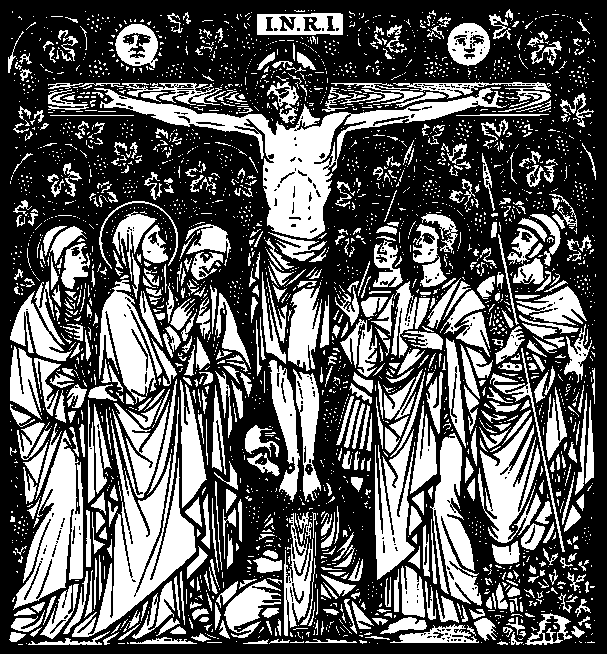
\includegraphics[width=0.44\textwidth]{../Images/Friday.pdf}
\end{center}
\vfill
